\section{Flachfundationen}
\begin{minipage}{0.8\linewidth}
	\subsection{Tragfähigkeit}
		\begin{tabular}{|l|l|l|}
			\hline
			Formel			&	Einheit		&	Bemerkung \\ \hline
			
			$ R_n
			= \bar{a} \cdot \bar{b} \cdot \sigma $ & [kN] & Achtung: Formel gilt für $ d/b \leq 2 $ \\ 
			$ \bar{a}
			= a - 2 \cdot e_a $ &	[m]		& reduzierter QS-Wert	\\
			$ e_a
			= \frac{M_y}{F_z} $ &	[m]		& Exzentrizität	\\
			$ \bar{b}
			= b - 2 \cdot e_b $ &	[m]		& reduzierter QS-Wert	\\
			$ e_b
			= \frac{M_x}{F_z} $ &	[m]		& Exzentrizität	\\
			$ \sigma_{\gamma}
			= \gamma_2 \cdot \bar{b} \cdot N_b + ( \gamma_1 \cdot d + q ) \cdot N_d + c \cdot N_c $	& $ \left[\frac{kN}{m^3}\right] $ / [kPa]	&	c = Kohäsion \\		\hline
%			$ N_b
%			= N_{b0} \cdot \nu_b \cdot \iota_b \cdot \lambda_b \cdot \xi_b $
%			& $ \left[\frac{kN}{m^3}\right] $		&	\\
%			$ N_{b0}
%			= ( N_{d0} - 1 ) \cdot tan (\varphi) $ & [kN]	& undrainiert: $ N_{b0} = 0 $\\
%			$ N_d
%			= N_{d0} \cdot \nu_d \cdot \iota_d \cdot \lambda_d \cdot \xi_d $
%							& $ \left[\frac{kN}{m^3}\right] $		&	\\
%			$ N_{d0}
%			= e^{ \pi \cdot tan ( \varphi) } \cdot tan^2 ( 45° + \frac{\varphi}{2} ) $ & [kN]	& undrainiert: $ \varphi_u = 0 $;  $ N_{d0} = 1 $ \\
%						&		& drainier: $ \varphi ' > 0 $ 	\\
%			$ \nu_d
%			= 1 + \frac{\bar{b}}{\bar{a}} \cdot \sin(\varphi) $ &			&	\\
%			$ \iota_d
%			= ( 1 - tan(\delta))^m $	&		&	\\
%			$ \delta
%			= arctan \left( \frac{T}{F_z}\right) $		 & $\degree$		& 3 dimensionaler Winkel	\\
%			$ T
%			= \sqrt{F_x^2 + F_y^2} $ & $ \left[\frac{kN}{m^3}\right] $ &	Resultierende \\	
%			$ m
%			= m_a \cdot cos^2 (\omega) + m_b \cdot sin^2 (\omega) $ & &	\\
%			$ m_a
%			= \frac{2 + \frac{\bar{a}}{\bar{b}}}{1 + \frac{\bar{a}}{\bar{b}}} $ & & \\
%			$ m_b
%			= \frac{2 + \frac{\bar{b}}{\bar{a}}}{1 + \frac{\bar{b}}{\bar{a}}} $ & & \\	
%			$ \omega
%			= arctan \left[ \frac{F_y}{F_x} \right] $ &  & \\
%			$ \lambda_d
%			= 1 - 0.4 \cdot tan ( \beta ) $ &		&	\\ 
%			$ N_c
%			= N_{c0} \cdot \nu_c \cdot \iota_c \cdot \lambda_c \cdot \xi_c $
%			& $ \left[\frac{kN}{m^3}\right] $		&	\\
%			$ N_{c0}
%			= ( N_{d0} - 1) \cdot cot (\varphi) $ & [kN]	& undrainiert: $ N_{c0} = 2 + \pi $ \\ \hline
		\end{tabular}
	
\end{minipage}
\begin{minipage}{0.25\linewidth}
	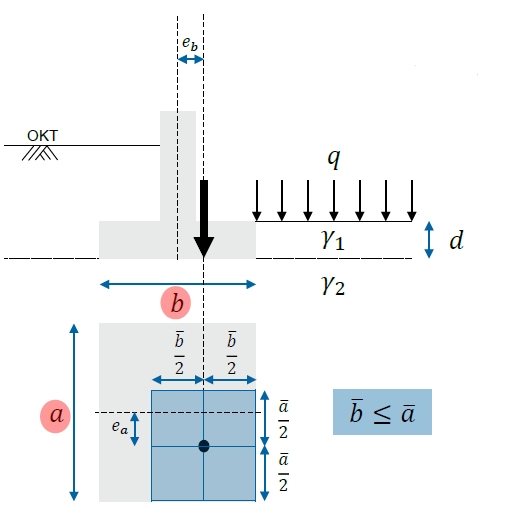
\includegraphics[width=\linewidth]{images/Flachfun1allgTragfah.PNG}
\end{minipage}


\begin{minipage}{0.85\linewidth}
	\begin{tabular}{l|l|ll}
		Bemerkung	& drainiert $ \varphi ' > 0 $	& undrainiert $ \varphi_u = 0 $ & \\ \hline
		
		Tragfähigkeitbeiwerte	& $ N_b
									= N_{b0} \cdot \nu_b \cdot \iota_b \cdot \lambda_b \cdot \xi_b $											& &	\\
								& $ N_d
								= N_{d0} \cdot \nu_d \cdot \iota_d \cdot \lambda_d \cdot \xi_d $	& & \\
								& $ N_c
								= N_{c0} \cdot \nu_c \cdot \iota_c \cdot \lambda_c \cdot \xi_c $ & & \\ \hline
								& $ N_{b0}
								= ( N_{d0} - 1 ) \cdot tan (\varphi) $	& $ N_{b0} = 0 $ & \\
								& $ N_{d0}
								= e^{ \pi \cdot tan ( \varphi) } \cdot tan^2 ( 45° + \frac{\varphi}{2} ) $ & $ N_{d0} = 1 $ & \\
								& $ N_{c0}
								= ( N_{d0} - 1) \cdot cot (\varphi) $ & $ N_{c0} = 2 + \pi $ & \\ \hline
		Formbeiwert				& $ \nu_b
								= 1 - 0.3 \cdot \frac{\bar{b}}{\bar{a}} $	& $ \nu_b = 1 $ & \\
								& $ \nu_d
								= 1 + \frac{\bar{b}}{\bar{a}} \cdot \sin(\varphi) $ & $ \nu_d = 1 $ & \\
								& $ \nu_c = \frac{\nu_d \cdot N_{d0} -1}{N_{d0} -1} $ & $ \nu_c = 1 + 0.2 \cdot \frac{\bar{b}}{\bar{a}} $ & \\ \hline
		Lastneigungsbeiwert $ \delta > 0 $		& $ \iota_b = (1 - tan ( \delta [\degree] ) ) ^{(m+1)} $	& & \\
								& $ \iota_d = (1 - tan ( \delta [\degree] ) ) ^m $	& $ \iota_d = 1 $  & \\
								& $ \iota_c = \frac{\iota_d \cdot N_{d0} -1}{N_{d0} -1} $ & $ \iota_c = \frac{1}{2} + \frac{1}{2} \cdot \sqrt{1 - \frac{T}{\bar{a} \cdot \bar{b} \cdot c_u}} $ & 					% 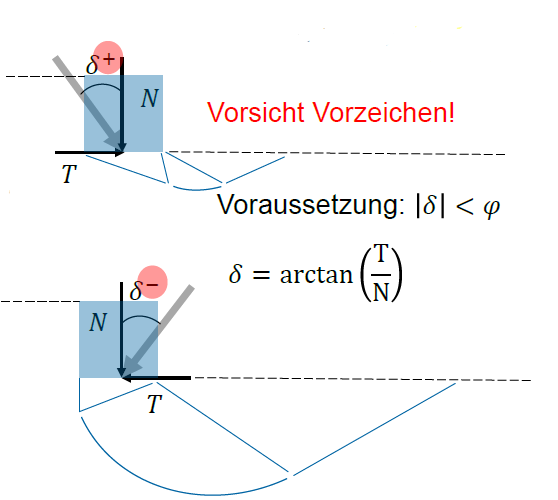
\includegraphics[width=0.2\linewidth]{images/Flachfun2Vorz.PNG} 
								\\
		Lastneigungsbeiwert $ \delta > 0 $ 	& $ \iota_b = cos ( \delta [\degree] ) \cdot (1 - 0.4 \cdot \delta [\degree]) ^{(0.64 + 0.028 \cdot \varphi [\degree])} $ & & \\
								& $ \iota_d = cos (\delta [\degree]) \cdot (1 - 0.0244 \cdot \delta [\degree]) ^{(0.03 + 0.04 \cdot \varphi [\degree])} $ & & \\
								& $ \iota_c = \frac{\iota_d \cdot N_{d0} -1}{N_{d0} -1} $ & & \\
								&&& \\
		3 dimensionaler Winkel	& $ \delta = arctan \left( \frac{T}{F_z}\right) $		 & 	& 	\\
		Resultierende			& $ T = \sqrt{F_x^2 + F_y^2} $ &  &	 \\
								& $ m = m_a \cdot cos^2 (\omega) + m_b \cdot sin^2 (\omega) $ & & \\
								& $ \omega = arctan \left[ \frac{F_y}{F_x} \right] $ &  & \\
								& $ m_a = \frac{2 + \frac{\bar{a}}{\bar{b}}}{1 + \frac{\bar{a}}{\bar{b}}} $ & & \\
								& $ m_b = \frac{2 + \frac{\bar{b}}{\bar{a}}}{1 + \frac{\bar{b}}{\bar{a}}} $ & & % 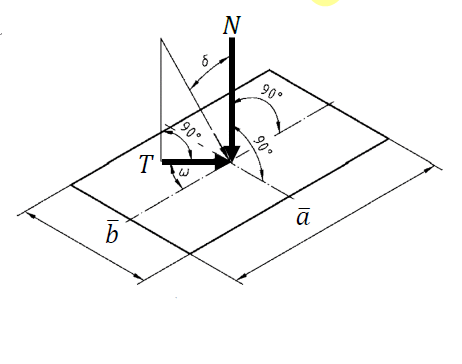
\includegraphics[width=0.2\linewidth]{images/Flachfun2Winkel.PNG} 
								\\ \hline
		Geländeneigungsbeiwert & $ \lambda_b = (1 - \frac{1}{2} \cdot tan (\beta [\degree] ) ) ^6 $ 	& & \\
								& $ \lambda_d = (1 - tan (\beta [\degree] ) ) ^{1.9} $	& $ \lambda_d = 1 $ & \\
								& $ \lambda_c = \frac{N_{d0} \cdot e ^{ (-0.0349 \cdot \beta [°] \cdot tan (\varphi [\degree] ) ) } -1 }{N_{d0} - 1} $	& $ \lambda_c = 1- 0.4 \cdot tan ( \beta [\degree] ) $ \\
								&	& $ \rightarrow $wenn $ \beta < \varphi $ & %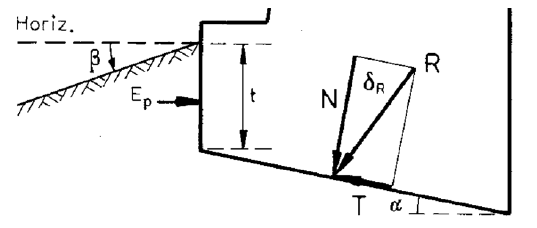
\includegraphics[width=0.2\linewidth]{images/Flachfun3Neig.PNG}
								\\ \hline 
		Sohlneigungsbeiwert		& $ \xi_b = e ^{(-0.045 \cdot \alpha [\degree] \cdot tan (\varphi [\degree]))} $	&	& \\
								& $ \xi_d = e ^{(-0.045 \cdot \alpha [\degree] \cdot tan (\varphi [\degree]))} $	& $ \xi_d = 1 $ & \\
								& $ \xi_c = e ^{(-0.045 \cdot \alpha [\degree] \cdot tan (\varphi [\degree]))} $ & $ \xi_c = 1 - 0.0068 \cdot \alpha [\degree] $ & %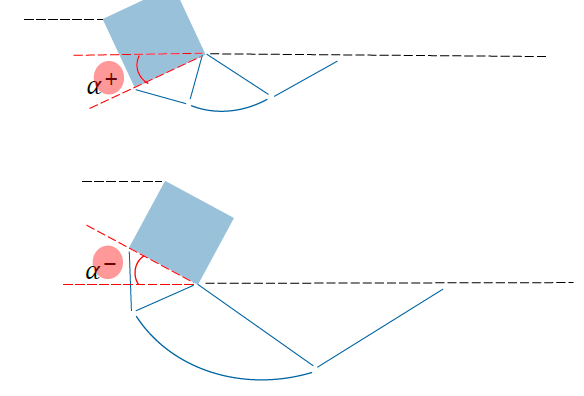
\includegraphics[width=0.2\linewidth]{images/Flachfun4Winkel.PNG} 
								\\ \hline			
		
	\end{tabular}
\end{minipage}
\begin{minipage}{0.2\linewidth}
	
	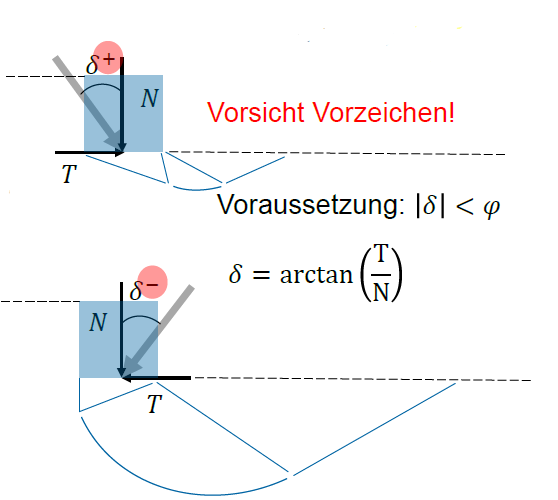
\includegraphics[width=\linewidth]{images/Flachfun2Vorz.PNG} \\
	
	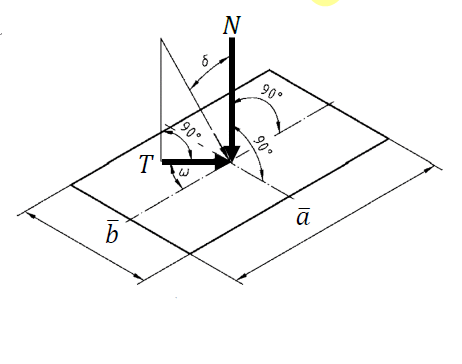
\includegraphics[width=\linewidth]{images/Flachfun2Winkel.PNG} \\
	
	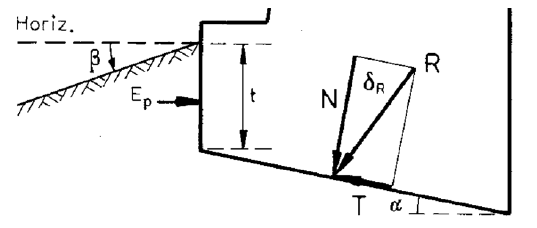
\includegraphics[width=\linewidth]{images/Flachfun3Neig.PNG} \\
	
	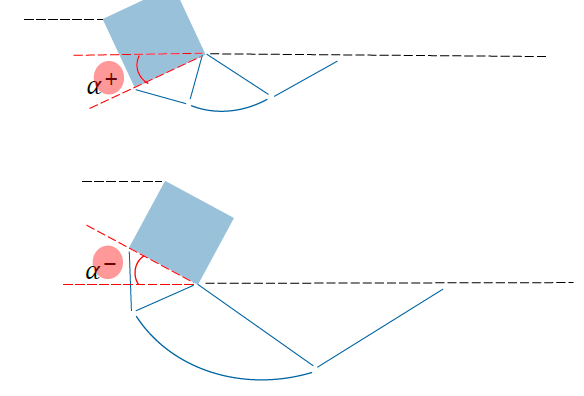
\includegraphics[width=\linewidth]{images/Flachfun4Winkel.PNG} \\
	
\end{minipage}


\textcolor{red}{Statistik, Berechnungswert $ \varphi_d $, Sicherheitsbeiwerte Geotech}



	\begin{minipage}{\linewidth}
		\subsection{Gebrauchstauglichkeit}
	
	

	\end{minipage}



\begin{minipage}{\linewidth}
	\begin{tabular}{l|l|l}
		Formel			&	Einheit	&	Bemerkung \\ \hline
	\end{tabular}
\end{minipage}